\documentclass[12pt]{article}
\usepackage[french]{babel}
\usepackage{natbib}
\usepackage{url}
\usepackage[utf8x]{inputenc}
\usepackage{amsmath}
\usepackage{graphicx}
\usepackage[svgnames]{xcolor}
\usepackage{vmargin}
\setmarginsrb{3 cm}{1 cm}{3 cm}{1.5 cm}{1 cm}{0.5 cm}{1 cm}{1.5 cm}
\usepackage{multirow}
\graphicspath{{images/}}
\usepackage{parskip}
\usepackage{fancyhdr}
\usepackage[T1]{fontenc}
\usepackage{url}
\usepackage{pdfpages}
\usepackage{url}
\usepackage{hyperref}
\usepackage{graphicx}
\usepackage{subcaption}
\usepackage{empheq, cases}
\usepackage{amssymb}
\usepackage{amsmath}
\usepackage{verbatimbox}
\usepackage{tcolorbox}
\usepackage{float}
\usepackage{multicol}
\usepackage[compact]{titlesec}
\usepackage[colorinlistoftodos]{todonotes}






\xdefinecolor{gray}{named}{lightgray}
\xdefinecolor{alice}{named}{AliceBlue}
\xdefinecolor{saumon}{named}{PeachPuff}
\definecolor{myred1}{RGB}{255, 0, 0}
\definecolor{mygreen1}{RGB}{0, 126, 0}
\definecolor{myblue1}{RGB}{0, 0, 61}
\definecolor{lightgray}{rgb}{0.83, 0.83, 0.83}
\definecolor{brick}{rgb}{0, 0, 0.50}

\tcbset{colback=lightgray,colframe=black}



\title{\color{brick} Optimisation TD 2:\\
\LARGE{Régression non linéaire et méthode de levenberg Marquardt}}								% Title
\author{Émilie Mathian}								% Author
\date{Année 2018 - 2019}											% Date

\makeatletter
\let\thetitle\@title
\let\theauthor\@author
\let\thedate\@date
\makeatother

\pagestyle{fancy}
\fancyhf{}
\rhead{\theauthor}
\lhead{Optimisation TD 1}
\cfoot{\thepage}
%%%%%%%%%%%%%%%%%%%%%%%%%%%%%%%%%%%%%%%%%%%%%%%%%%%%%%%%%%%%%%%
\usepackage{eso-pic}
\newcommand\BackgroundPic{%
\put(0,0){%
\parbox[b][\paperheight]{\paperwidth}{%
\vfill
\centering
\includegraphics[width=\paperwidth,height=\paperheight,%
keepaspectratio]{background.png}%
\vfill
}}}
  
  
\begin{document}

%%%%%%%%%%%%%%%%%%%%%%%%%%%%%%%%%%%%%%%%%%%%%%%%%%%%%%%%%%%%%%%%%%%%%%%%%%%%%%%%%%%%%%%%%

\begin{titlepage}
	\centering
    \vspace*{0.5 cm}
    \vspace{-3.5cm}
    
\includegraphics[width = 4cm]{logo.png}\\	% University Logo
    \textsc{\LARGE Institut National des Sciences Appliquées de Lyon}\\[2.0 cm]	% University Name
	\textsc{\Large $4^{eme}$ Année Bioinformatique et Modélisation}\\[0.5 cm]				% Course Code
	\textsc{\large Professeur: Noëlie DEBS }\\[0.5 cm]				% Course Name
	\rule{\linewidth}{0.2 mm} \\[0.4 cm]
	{ \huge \bfseries \thetitle}\\
	\rule{\linewidth}{0.2 mm} \\[1.5 cm]
	
	\begin{minipage}{0.4\textwidth}
		\begin{flushleft} \large
			\emph{Auteur:}
			\theauthor
			\end{flushleft}
			\end{minipage}~
			\begin{minipage}{0.4\textwidth}	
	\end{minipage}\\[2 cm]
    \vspace{-1.8cm}
	 \begin{figure}[H]
	\begin{center}
	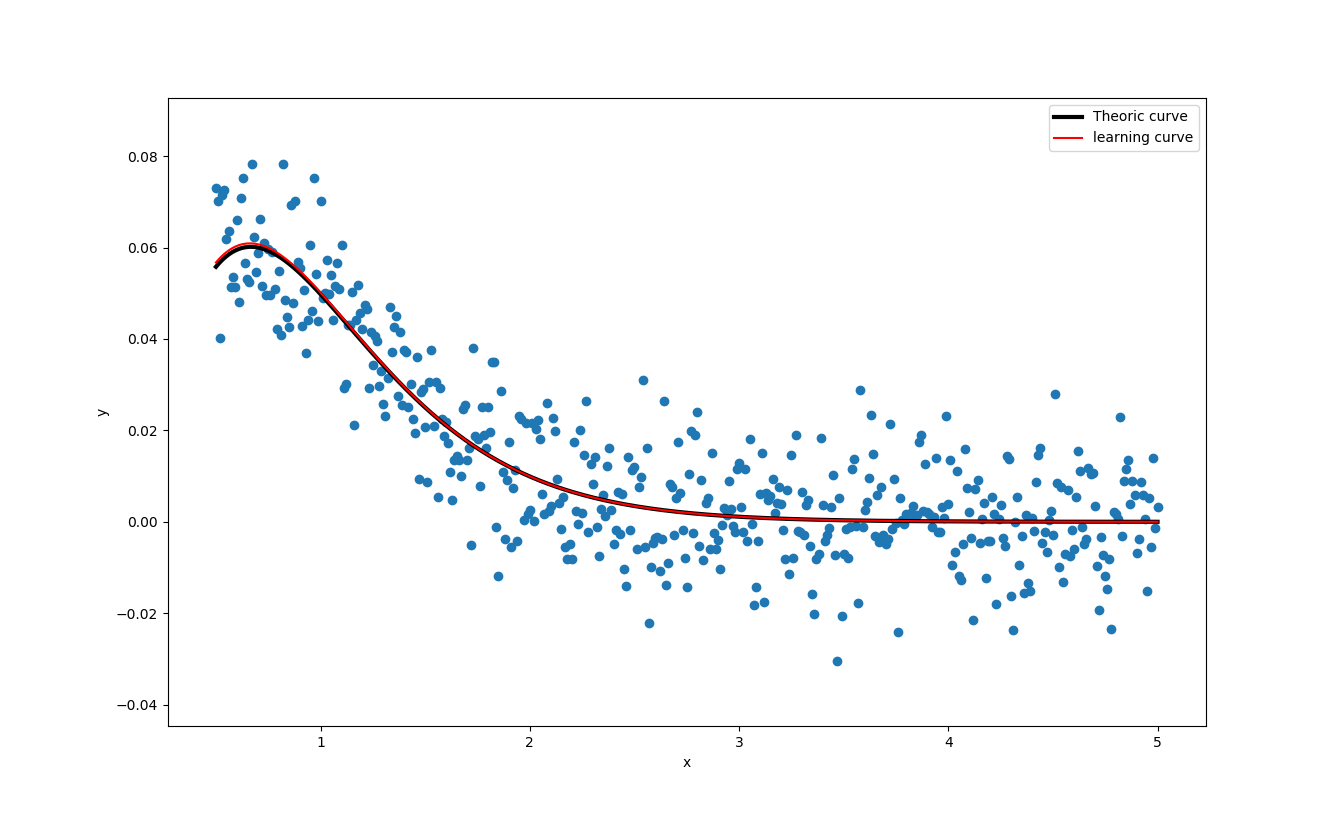
\includegraphics[width=0.65 \textwidth]{Figure_1.png}
\end{center}
\end{figure}

	{\large \thedate}\\[1 cm]
    
	\vfill

 

\end{titlepage}
\pagebreak
%%%%%%%%%%%%%%%%%%%%%%%%%%%%%%%%%%%%%%%%%%%%%%%%%%%%%%%%%%%%%%%%%%%%%%%%%%%%%%%%%%



\newpage 


\newpage

\begin{center}
\fcolorbox{black}{lightgray}{
\begin{minipage}{\linewidth}
\textbf{Problématique :} \\
L'objectif de ce TD est d'implémenter la méthode de Levenberg Marquardt. Cette algorithme, dans le contexte de la régression non linéaire, permet  d'obtenir une estimation optimale des paramètres de l'équation telle que la somme des carrés des écarts soit minimisée. L'ensemble du programmme est contenu dans le fichier "TP2\_opt.py", l'ensemble des questions sonnt référencées dans le "Main" du programme. \\
\textit{Nb : les normes sont calculées d'après la définition de normes euclidiennes telles que $||\vec{u}||= \sqrt{x^2 + y^2}$}
\end{minipage}}
\end{center}
\vspace{0.5cm}

\section*{\color{brick} Cas 1:  Fonction mono expoentielle}
\textbf{\color{brick}1.} 
Dans le TP précédent nous avions implémenter la méthode de descente de gradient, et nous avions constaté que cet algorithme est performant dans le sens où il garantit de converger vers un minimums. Néanmoins la méthode de descente de gradient impose de fixer un pas de converge $\alpha$ tel que $f(x_k+1) = f(x_k) - \alpha \nabla f $, il sera à l'utilisateur le soin d'optimiser le choix de ce paramètre. De plus cette méthode impose que $f$ soit de classe $\mathcal{C}^1$.\\
L'implémentation de la méthode de Newton nous a permis d'observer l'efficacité de l'algorithme étant donné sa vitesse de converge. Toutefois, l'algorithme de Newton ne distingue pas les maximums des minimums ni les points selle. De plus la méthode repose sur le calcul de la Hessienne, calcul coûteux qui impose que $f$ soit de classe $\mathcal{C}^2$.\\

\textbf{\color{brick}2.} La fonction g a pour expression : $g(x) = e ^{-ax}$. Le seul paramètre que nous devrons estimer est donc '$a$'. Le calcul de la fonction g a été implémenter tel que \verb|g (x,a)|, où les entrées sont : \verb|x|  un vecteur de dimension $(n,1)$, et \verb|a| une valeur pour le paramètre; la sortie est un vecteur \verb|y| de dimension $(n,1)$. \\


\textbf{\color{brick}3.} La fonction \verb|random\_data\_set(x,a,b)| permet de construire un jeu aléatoire de y points tels que  $y= g(a,x) +b \mathcal{N}(0,1)$. Ainsi pour tout x on calcul le résultats de la fonction $g(x)$ auquel on ajoute un résidu aléatoire tiré d'une lois normale que l'on pondère d'un facteur $b$.
\newpage

\textbf{\color{brick}4.} 
\begin{figure}[H]
\centering
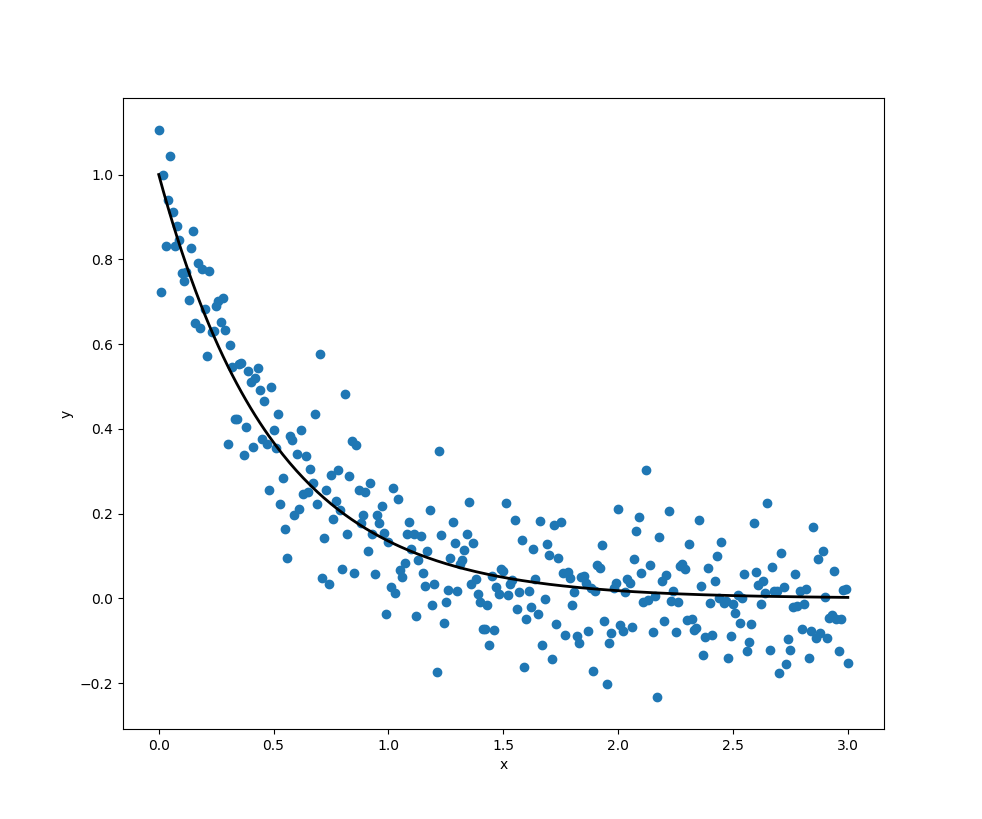
\includegraphics[width=0.8\textwidth]{Q4.png}
\caption{Génération d'un jeu de données aléatoire tel que $y= e^{-2x} + b \mathcal{N}(0,1) $ avec b=0.1, sur un intervalle $x\in[0,3$ avec un pas de 0.01. La courbe noir a pour équation $y= e^{-2x}$, c'est donc par construction la fonction qui minimise la SCE. }
\label{Fig1}
\end{figure}

\textbf{\color{brick}5.} La fonction de coût à minimiser, dans de régression linéaire n'est autre que la fonction de la somme des carrés des écarts entre les données empiriques et théoriques. $f$ s'écrit alors  pour notre cas telle que $f(a) \frac{1}{2}\sum_{i=1}^N(y_i - e^{-ax}) $.  Dans notre programme cettte fonction a été nomée \verb|cost_fucntion(x,y,a)|, qui d'après un vecteur de données $y$, un vecteur et selon un paramètre $a$ retourne la SCE.


\textbf{\color{brick}6.} La minimisation de la fonction $f$ d'après la méthode de Levenberg Marquardt utilise le gradient de la fonction de coût. La formule général du gradient est \\
$\frac{\partial f}{\partial a_k} = - \sum_{i=1}^N = (y_i - g(x_i,a))\frac{\partial g}{\partial a_k}(x_i,a) $  ce qui dans notre cas donne :
$$ \frac{\partial f}{\partial a} =\sum_{i=1}^N (y_i - e^{-ax_i}(x_ie^{-ax_i})) $$
Ainsi nous avons écris la fonction \verb|grad (x,y,a)|, qui prend en entrée le vecteur des données $y$ et un vecteur $x$ et un paramètre $a$  et retourne la valeur de la dérivée  pour une valeur de $a$ considéree.
 
\textbf{\color{brick}7.} La méthode de Levenberg Marquardt requiert également le calcul de la dérivée seconde, nous utiliserons ici l'approxiamtion de Gauss Newton pour simplifier les calculs. Rappelons que la formule générale est $\frac{\partial ^2 f }{\partial a_K \partial a_l} = \sum_{i=1}^N \frac{\partial g}{\partial a_k}g(x_i, \textbf{a})\frac{\partial g}{\partial a_l}g(x_i, \textbf{a})$, d'après notre fonction et sachant que nous n'avons qu'un paramètre à estimer nous obtenons :\\ 
\begin{align*}
    \frac{\partial ^2 f }{\partial a ^2} &=  \sum_{i=1}^N \frac{\partial g}{\partial a}g(x_i, a)\frac{\partial g}{\partial a}g(x_i, a)\\
    &= \sum_{i=1}^N ( \frac{\partial g}{\partial a}(x_i, a)^2) \\
    &=  \sum_{i=1}^N (-xe^{a-x})^2
\end{align*}
La fonction \verb|derivative_2 (x,a,l)| résout l'opération ci-dessus; rappelons que l'algorithme de Levenberg Maquardt permet de moduler l'importance de la dérivée seconde par la dérivée première en multipliant $ \frac{\partial ^2 f }{\partial a ^2} $ par un coefficient $(1= \lambda)$, c'est pourquoi  \verb|derivative_2| prend en entré le paramètre \verb|l| qui traduit $\lambda$. La fonction  retourne pour un $a$ et un $\lambda$ donnés le résultats de la dérivée seconde de la fonction de coût en fonction de la valeur estimé du paramètre $a$, pondérée par la valeur de $\lambda$.

\textbf{\color{brick}8.} Implémentation de l'algorithme de Levenberg Maquardt :\\
L'algorithme pour la fonction est nommé \verb|LM|, il prend en entrée les paramètres suivants :
\begin{itemize}
    \item \verb|x| un vecteur définissant l'intervalle de l'analyse
    \item \verb|y| un vecteur de données aléatoires (généré par \verb|random\_data\_set|)
    \item \verb|a| l'estimation initiale du paramètre
    \item \verb|l| une condition initiale du paramètre $\lambda$, coefficient modulant l'importance du gradient par rapport à la Hessienne lors du calcul de la direction.
    \item\verb|cond| qui est la condtition d'arrêt choisit qui d'après la fonction \verb|stop| peut les veleurs suivantes :
    \begin{itemize}
        \item 0 => condition d'arrêt par  rapport à un nombre maximal d'itérations donné par le paramètre \verb|k|
        \item 1 => condition d'arrêt par rapport à une norme minimale à atteindre donnée par le paramètre \verb|g|
        \item 2 => conditions d'arrêt relient le nombre d'itérations maximal et la norme minimale à atteindre
        \item 3 => condition d'arrêt impliquant que l'inéquation $f(a_{k+1})<f(a_k)$ soit vérifiée.
    \end{itemize}
\end{itemize}
A chaque itération l'algorithme \verb|LM| retourne la dernière  valeur de  $a$, la norme du gradient (\textit{ici équivalente à la valeur absolue de la dérivé première}), la fonction de coût dépendante de la dernière valeur calculée de $a$ dépendant elle même la direction calculée, notée \verb|dLM|. Rappelons en effet que  \verb|dLM|  est calculé telle que $dLM = -\frac{\nabla}{\nabla^2 f (1 + \lambda)}$ et que sa mise jour implique que  $a_{k+1} = a_k +dLM$. Soulignons par ailleurs que la mise jour de $a$ et $\lambda$ par rapport à \verb|dLM| dépend de vérification  de la condition $f(a_{k+1}) < f(a_k)$.

\textbf{\color{brick}9.} Nous allons étudier le comportement de l'algorithme \verb|LM| pour chaque itérations, avec les paramètres $g(x)= e{-2x}$ (d'où $a=2$) sur $x \in [0,3]$ et $b=0.01$.
\begin{figure}[H]
\centering
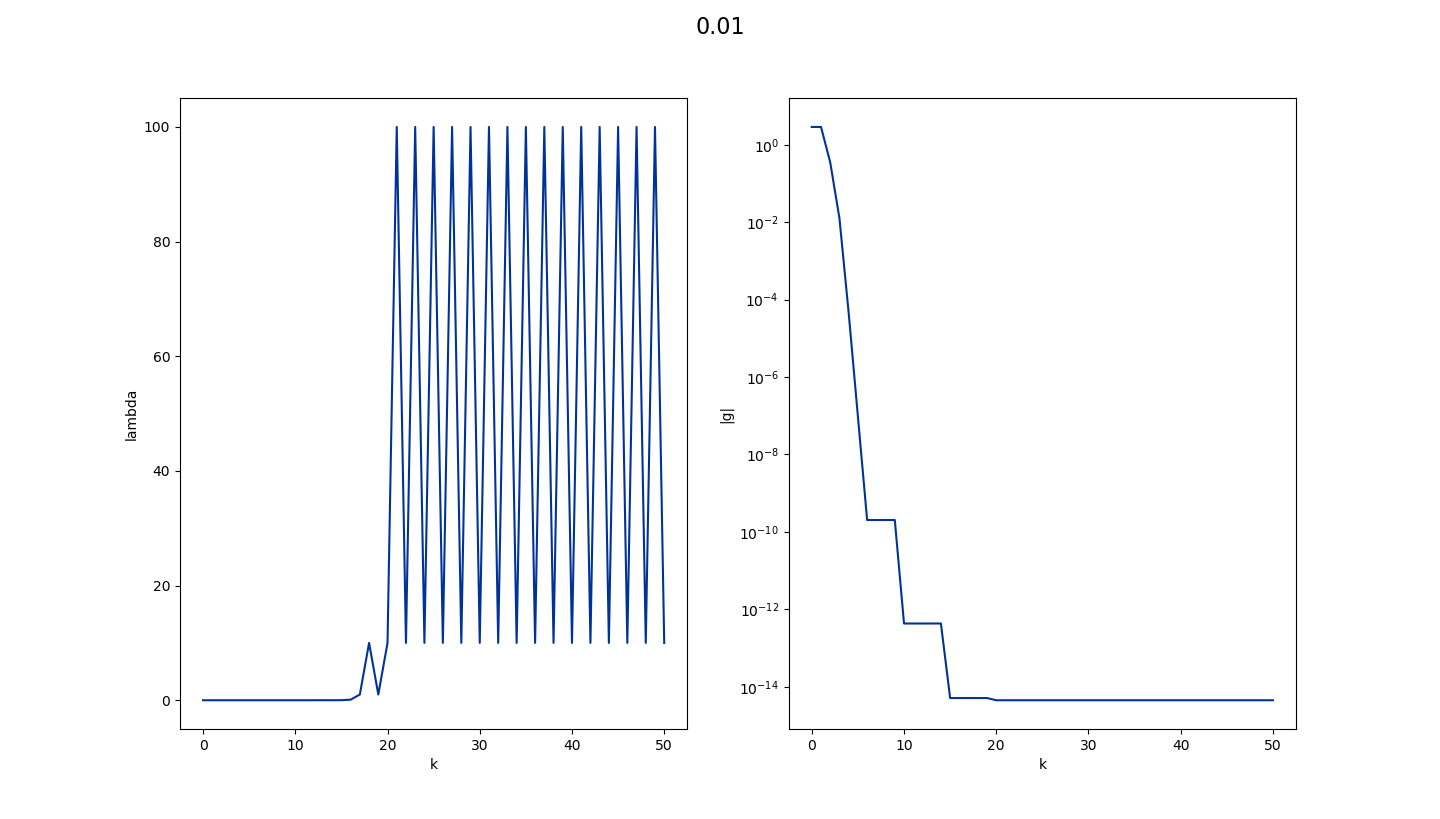
\includegraphics[width=0.9\textwidth]{Q0_L_G.png}
\caption{ À gauche nous suivons le comportement de $\lambda$, qui prend les valeurs successives de 10 ou  100. À droite nous l'évolution du logarithle de la norme du gradient.}
\label{FigQ9}
\end{figure}
Les opérations alternatives subies par $\lambda$ (multiplication, ou division) sont des indications de l'orientation prise par l'algorithme au cours des itérations. En effet rappelons que $\lambda$ est divisé lorsque qu'on privilège la direction d'ordre 1 et divisé lorsqu'on privilège la direction d'ordre 2. Ainsi l'algorithme utilise alternativement les deux méthodes.\\
Le gradient comme escompté décroît au cours des itérations, et coverge rapidement  vers une valeur très faible : $10^{-14}$.

\begin{figure}[H]
\centering
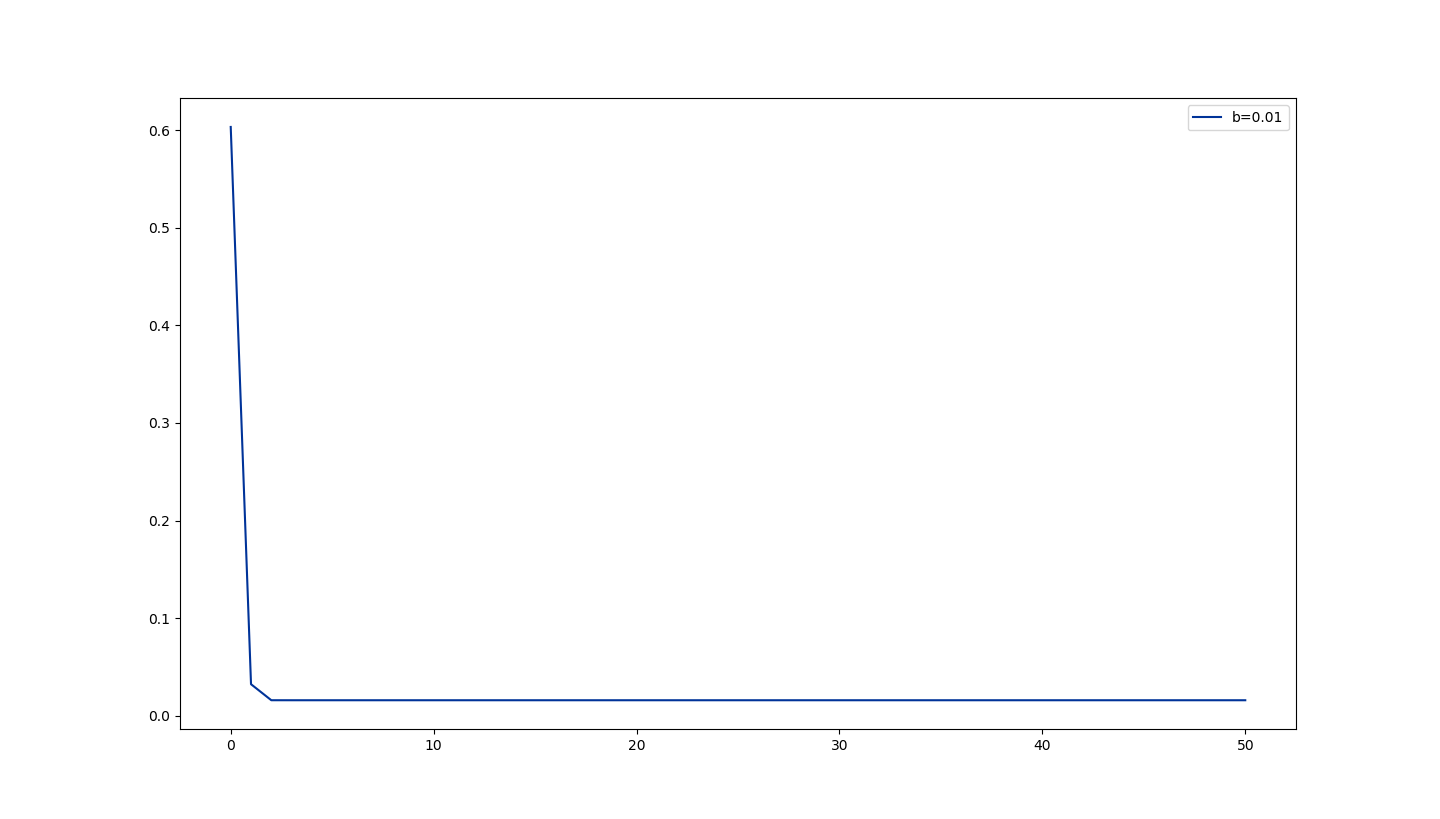
\includegraphics[width=0.9\textwidth]{Q9_F.png}
\caption{ Évolution de $f$ traduisant, l'évolution de SCE de notre modèle non linéaire. }
\label{FigQ9}
\end{figure}
 

Remarquons qu'ici pour une valeur du bruit est très faible $b=0.01$, ainsi la SCE à la fin du processus converge rapidement vers 0, ce qui ne serait pas le cas pour des données plus buritées.

\begin{figure}[H]
\centering
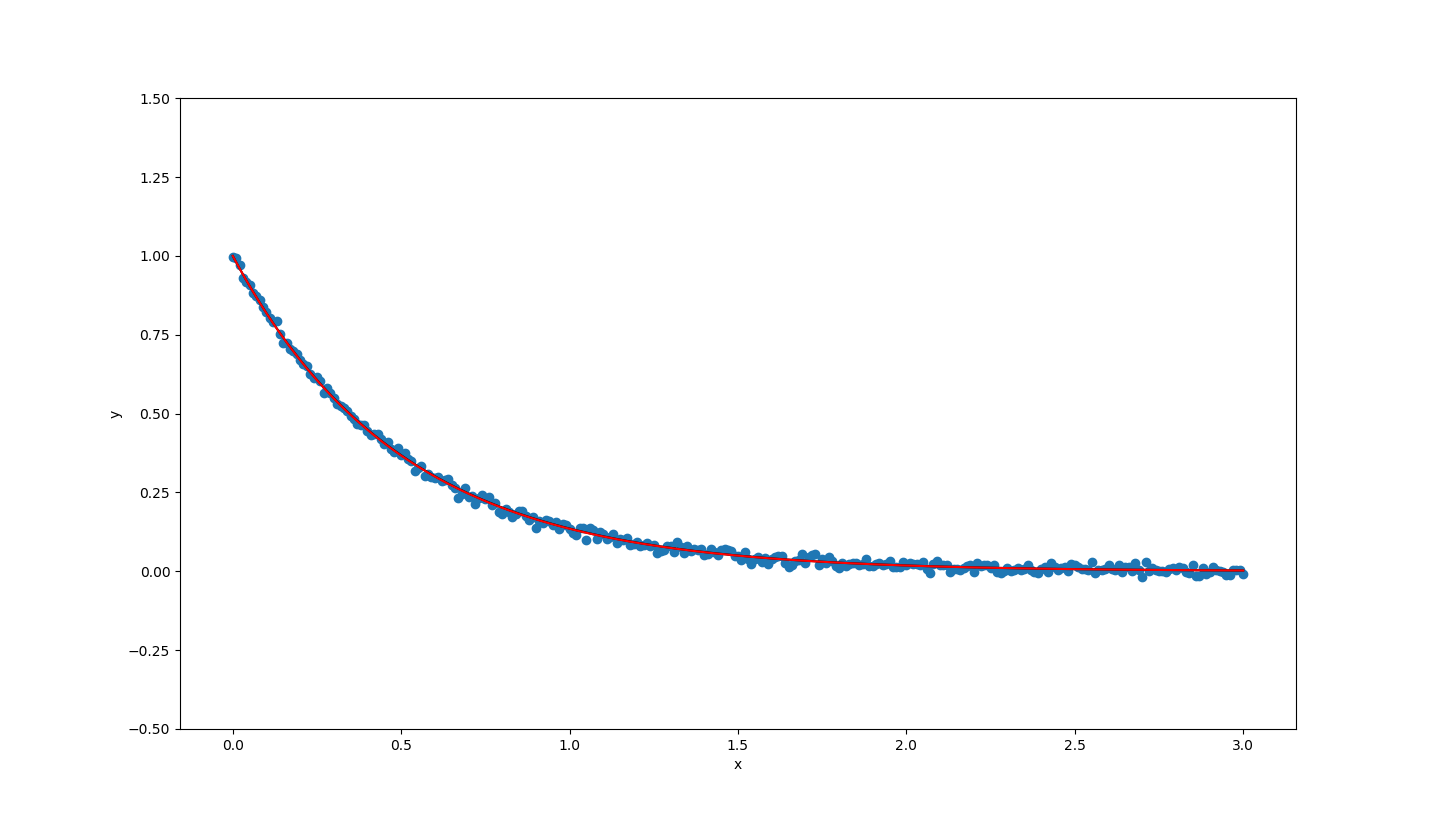
\includegraphics[width=0.9\textwidth]{Q9_S.png}
\caption{ En rouge apparaît les résultats du modèle prédit. On obtient au bout de 30 itération un $a \simeq 1.99 $ pour une valeur théorique de 2.}
\label{FigQ9}
\end{figure}
 
\textbf{\color{brick}10.} Nous à présent étudier l'effet du paramètre $b$ sur la convergence de l'algorithme \verb|LM|. Pour cela nous fixons $a=2$, nous travaillons un intervalle tel que $x \in [0,3]$ et nous prendrons les bruits $b=[0.01, 0.1 , 0.5 , 1]$. Nous obtenons les résultats suivants : 

\begin{figure}[H]
\centering
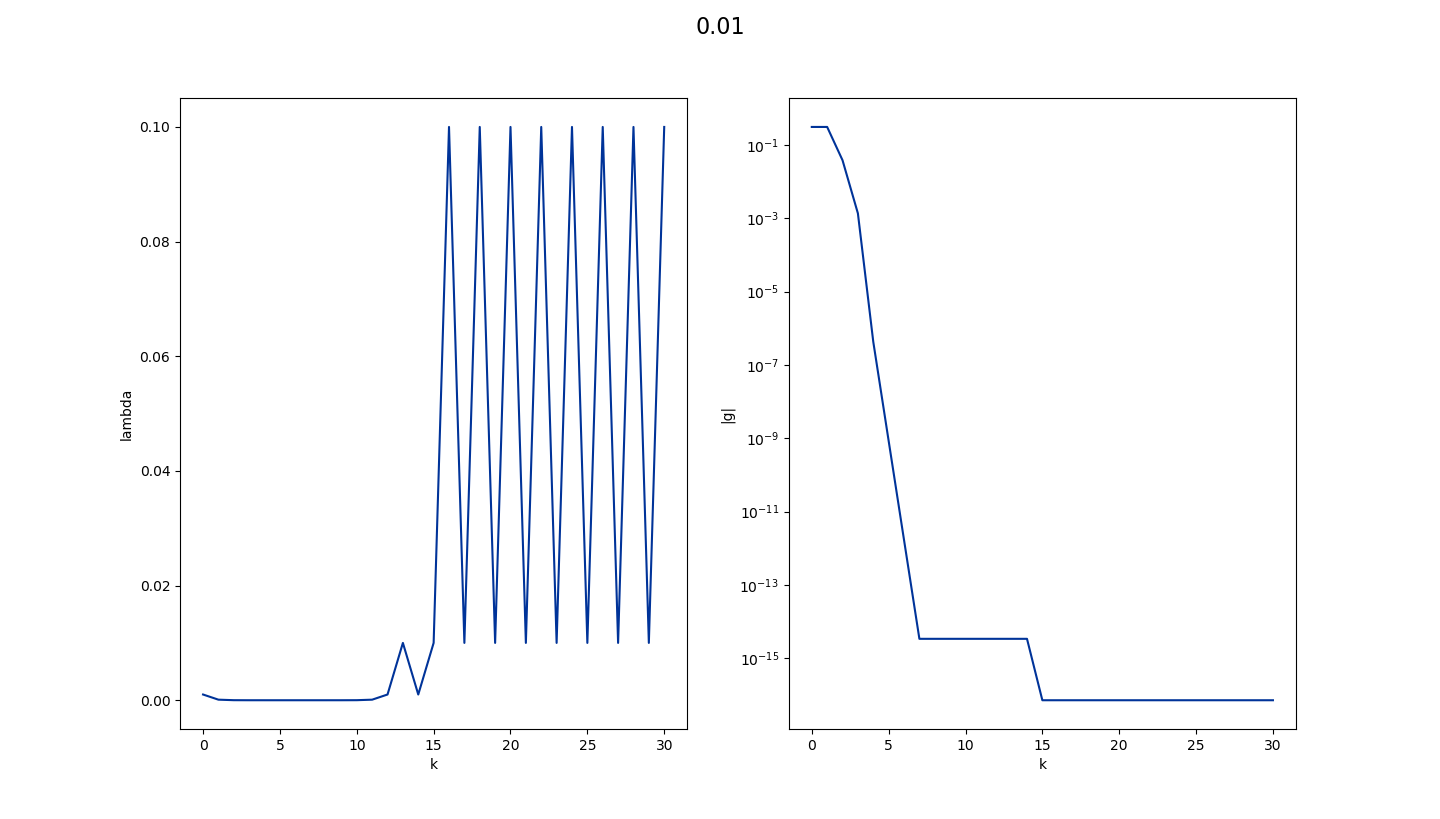
\includegraphics[width=0.7\textwidth]{Q10_B001.png}
\caption{ Évolution de $\lambda$ et de $|g|$ pour $b=0.O1$.}
\label{FigQ9}
\end{figure}


\begin{figure}[H]
\centering
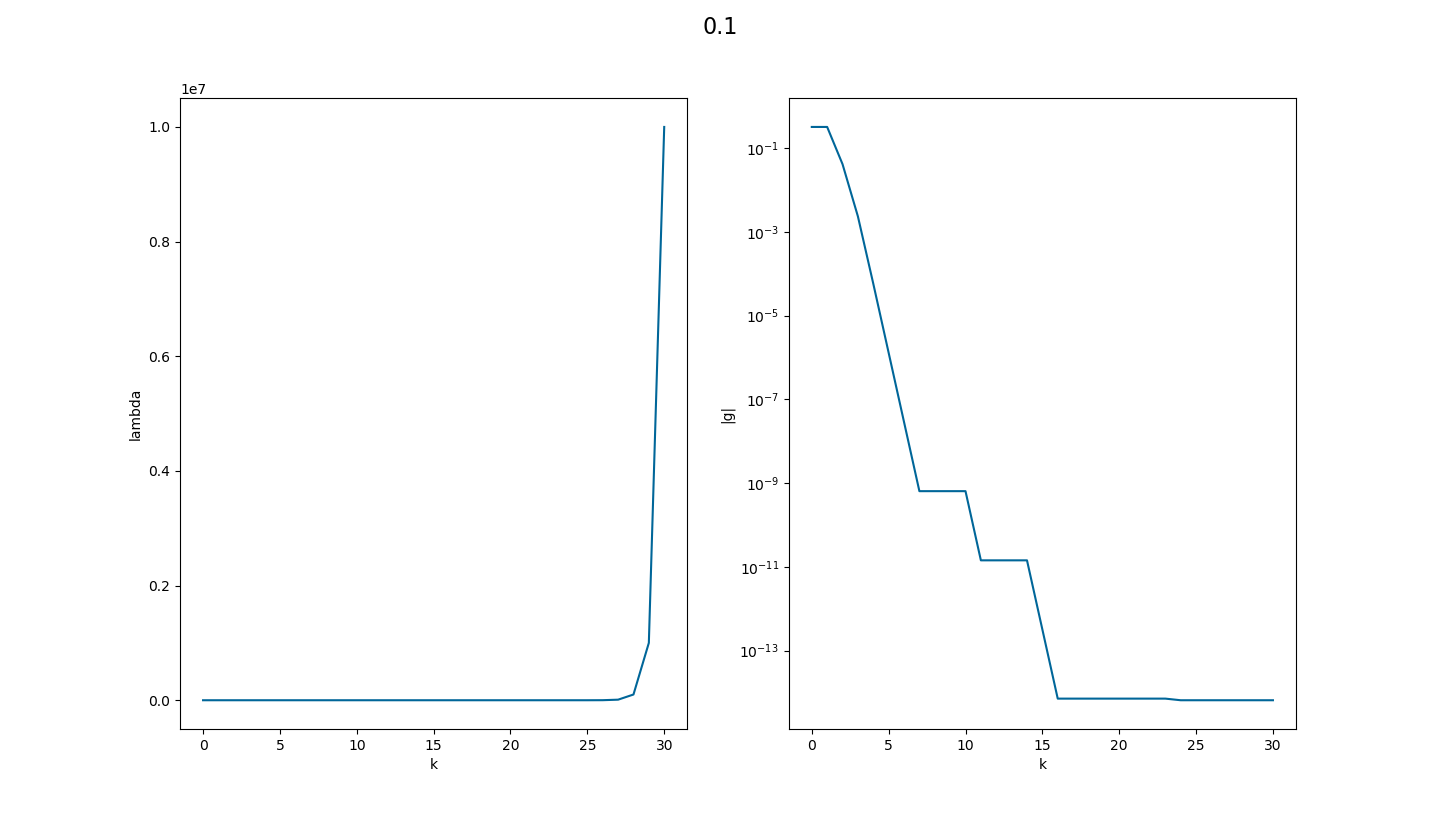
\includegraphics[width=0.7\textwidth]{Q10_B01.png}
\caption{ Évolution de $\lambda$ et de $|g|$ pour $b=0.1$.}
\label{FigQ10B01}
\end{figure}

\textit{Remarque : Dans le cas ci-dessus $\lambda$ a été multiplié à chaque itérations. Ainsi  les termes de la diagonale de la Hessienne sont prépondérants, donc la solution dépend principalement de la dérivée d'ordre 1.  }
% C'est juste



\begin{figure}[H]
\centering
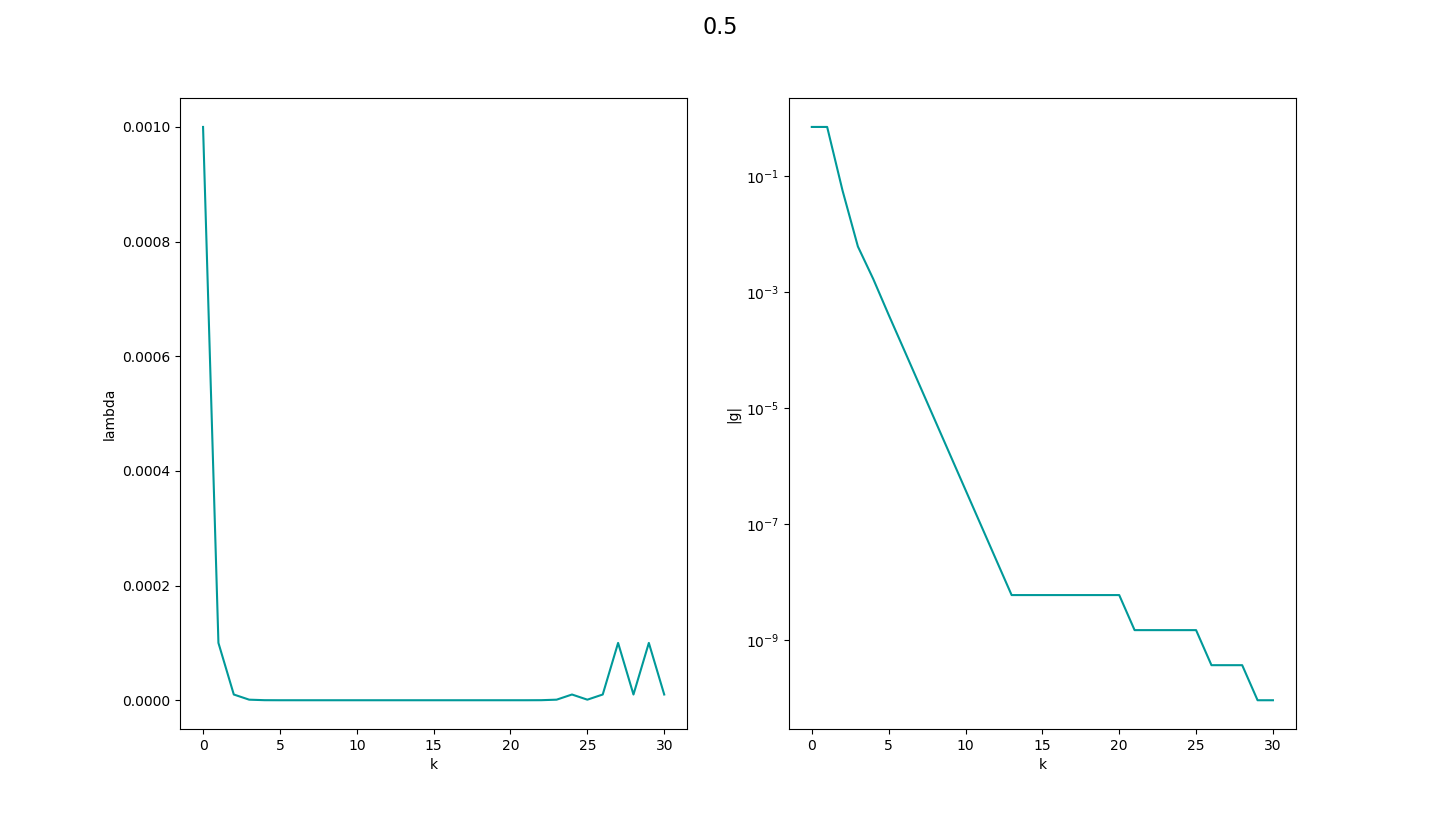
\includegraphics[width=0.7\textwidth]{Q10_B05.png}
\caption{ Évolution de $\lambda$ et de $|g|$ pour $b=0.5$.}
\label{FigQ10B01}
\end{figure}


\begin{figure}[H]
\centering
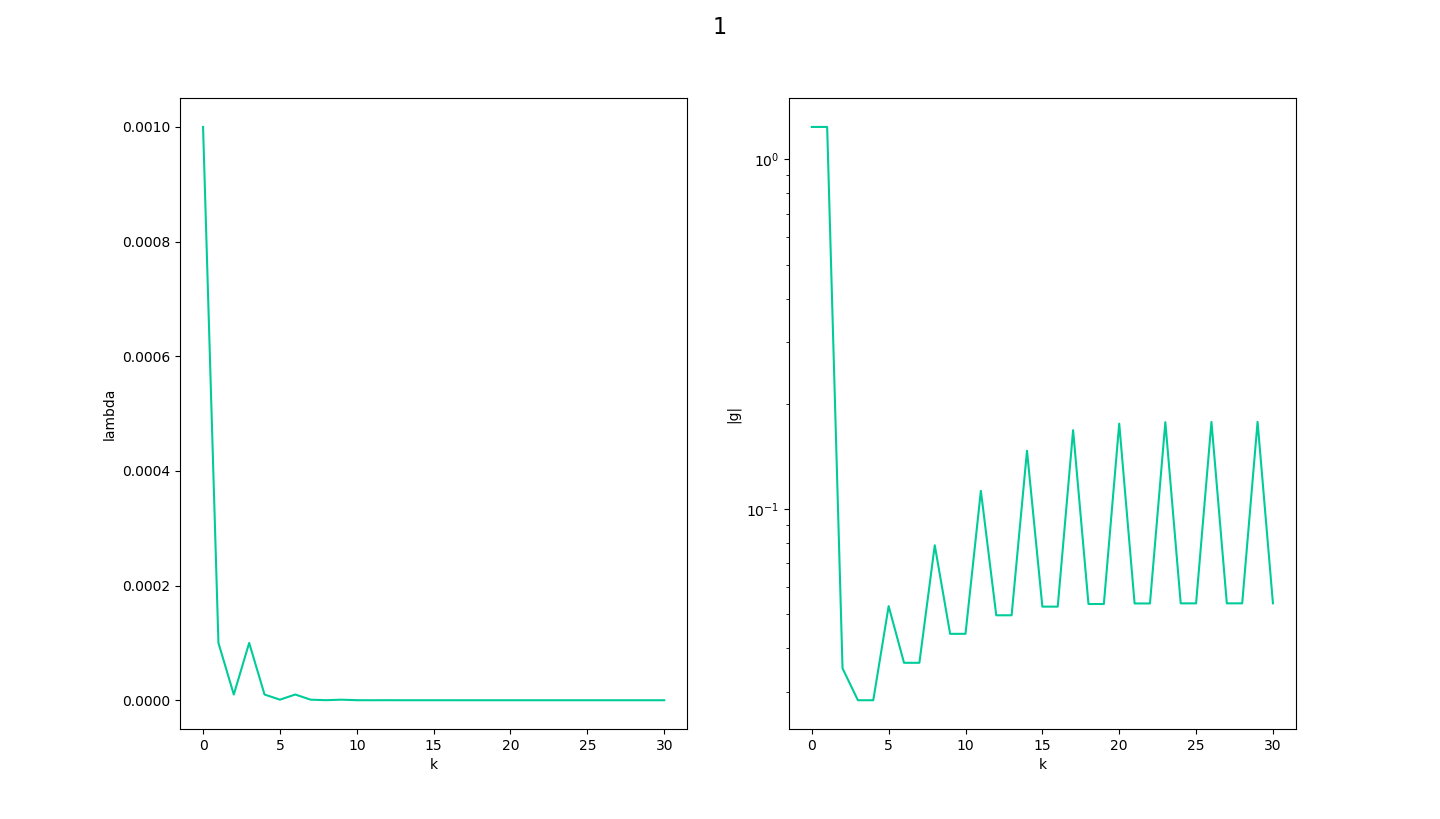
\includegraphics[width=0.7\textwidth]{Q10_B1.png}
\caption{ Évolution de $\lambda$ et de $|g|$ pour $b=1$.}
\label{FigQ10B01}
\end{figure}

D'après les graphiques précédents on constate que plus le bruit augmente moins la norme du gradient diminue. Le comportement de $\lambda$ est varie à la compilation est ne peut pas être facilement expliqué.


\begin{figure}[H]
\centering
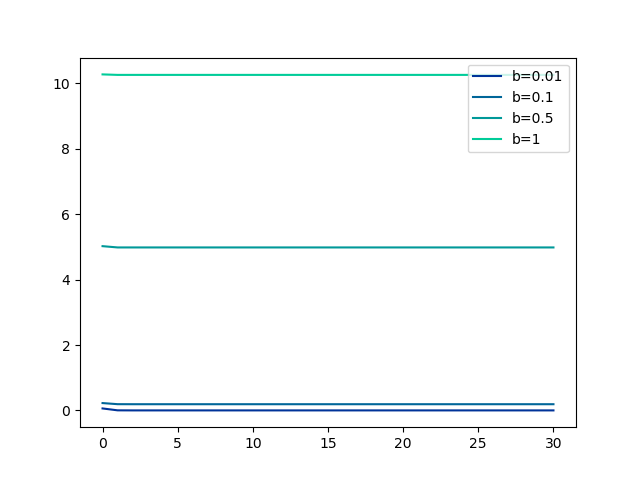
\includegraphics[width=0.7\textwidth]{Q10_F.png}
\caption{ Valeur de la fonction de coût en fonction du nombre d'itérations pour différentes valeurs de bruits.}
\label{FigQ10B01}
\end{figure}

D'après le graphique ci dessus, le minimum de la SCE est trouvé après un faible nombre d'ittérations. Ensuite la valeur se stabilise étant donné que $a$ est quasi cosntant. Par ailleurs l'augmentation induit une augmentation globale de la SCE.

\begin{figure}[H]
\centering
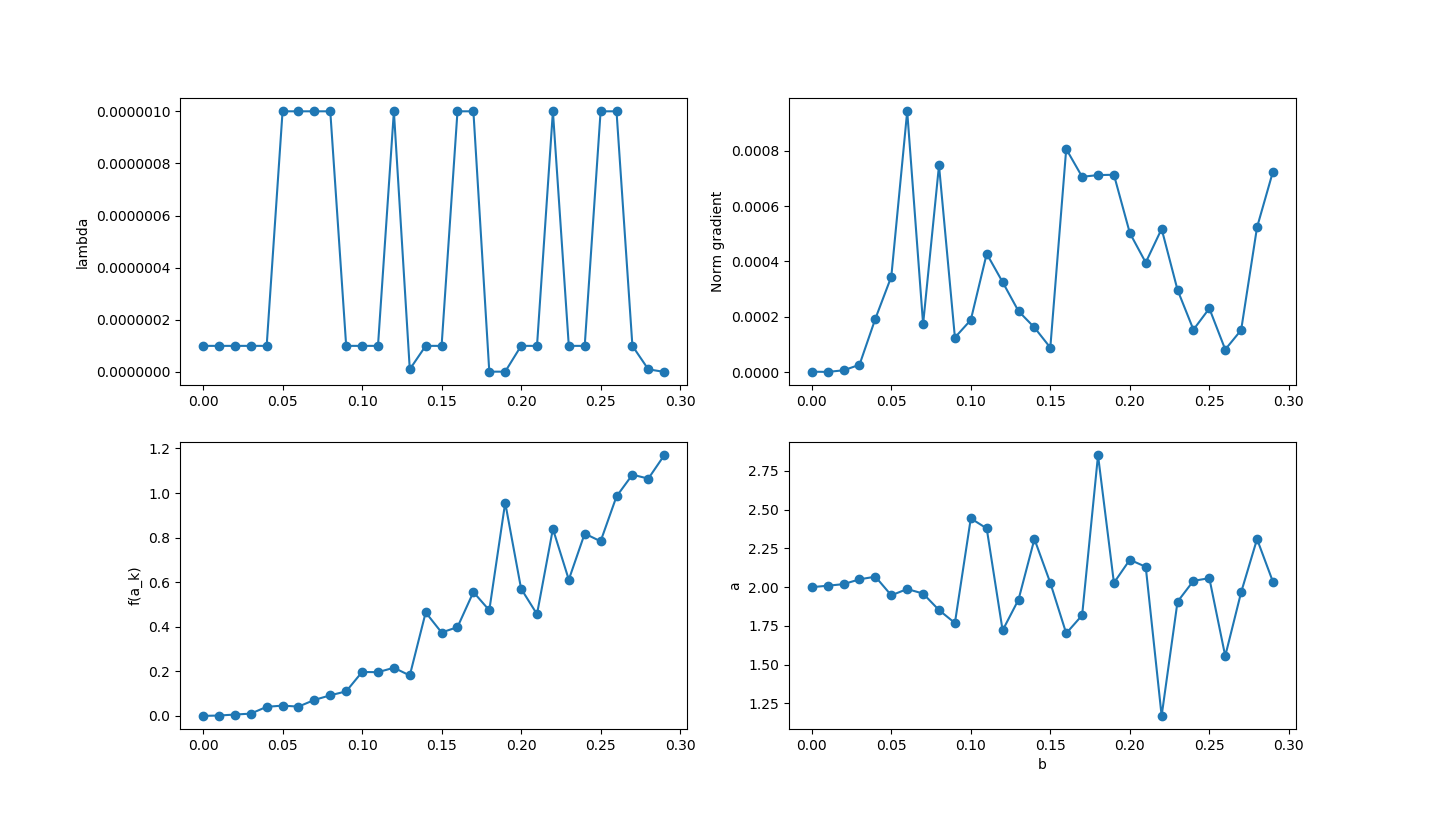
\includegraphics[width=1\textwidth]{Q10_E.png}
\caption{ Ébolution de $\lambda$, de $|g$, de $f(a_k)$ et de $a$ en fonction du bruit $b \in [0,0.3]$ avec un pas de 0.01 .}
\label{FigQ10B01}
\end{figure}
Ce graphique résume les informations précédentes, en effets nous observons que la SCE croit avec le bruit, ou encore que la norme du gradient d'après ue condition d'arrêt fixé sur le nombre d'itérations (k<30) reste faible mais devient instable lorsque b augmente. Enfin nous observons que l'approximation de $a$ est très proche du $a$ théorique si $b$ est faible, puis oscillle autour de la solution pour $b$ croissant.


\textbf{\color{brick}11.} Nous allons à présents tracer les données et les prédictions pour différentes valeur de $b$ testées :

\begin{figure}[H]
\centering
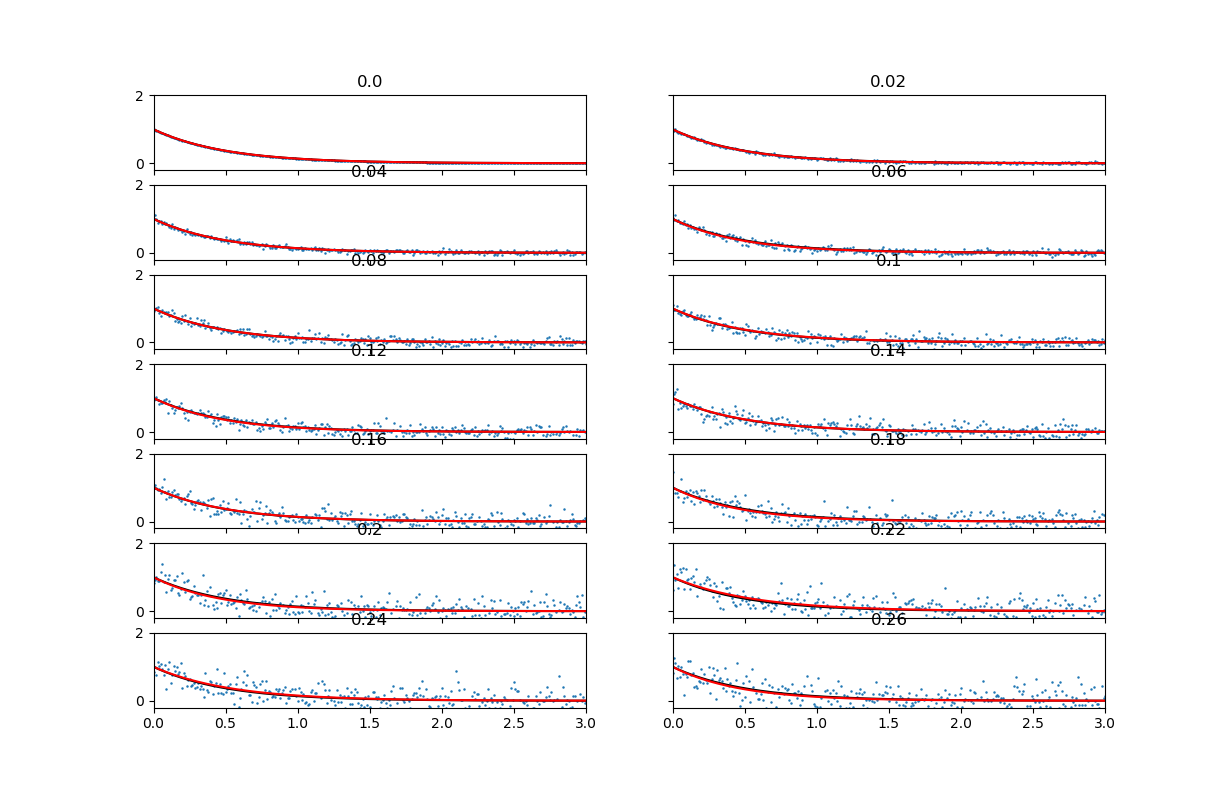
\includegraphics[width=1\textwidth]{Q111.png}
\caption{Données, courbe théorique (noire) et simulée (rouge) pour $a=2$ et différentes valeurs de $b  \in [0,3]$ par 0.1.}
\label{FigQ111}
\end{figure}

 D'après les graphiques ci-dessus [\ref{FigQ111}] la courbe simulée concorde parfaitement avec la courbe théorique et donc par construction minimise l'écart aux données. Ainsi pour les valeurs de $b$ ($b \in [0, 0.3]$) testées il est difficile de mettre en évidence une différence de la qualité de la modélisation en fonction du bruit. Nous essayons donc des valeurs de $b$ supérieure pour observer une différence : 
 
 \begin{figure}[H]
\centering
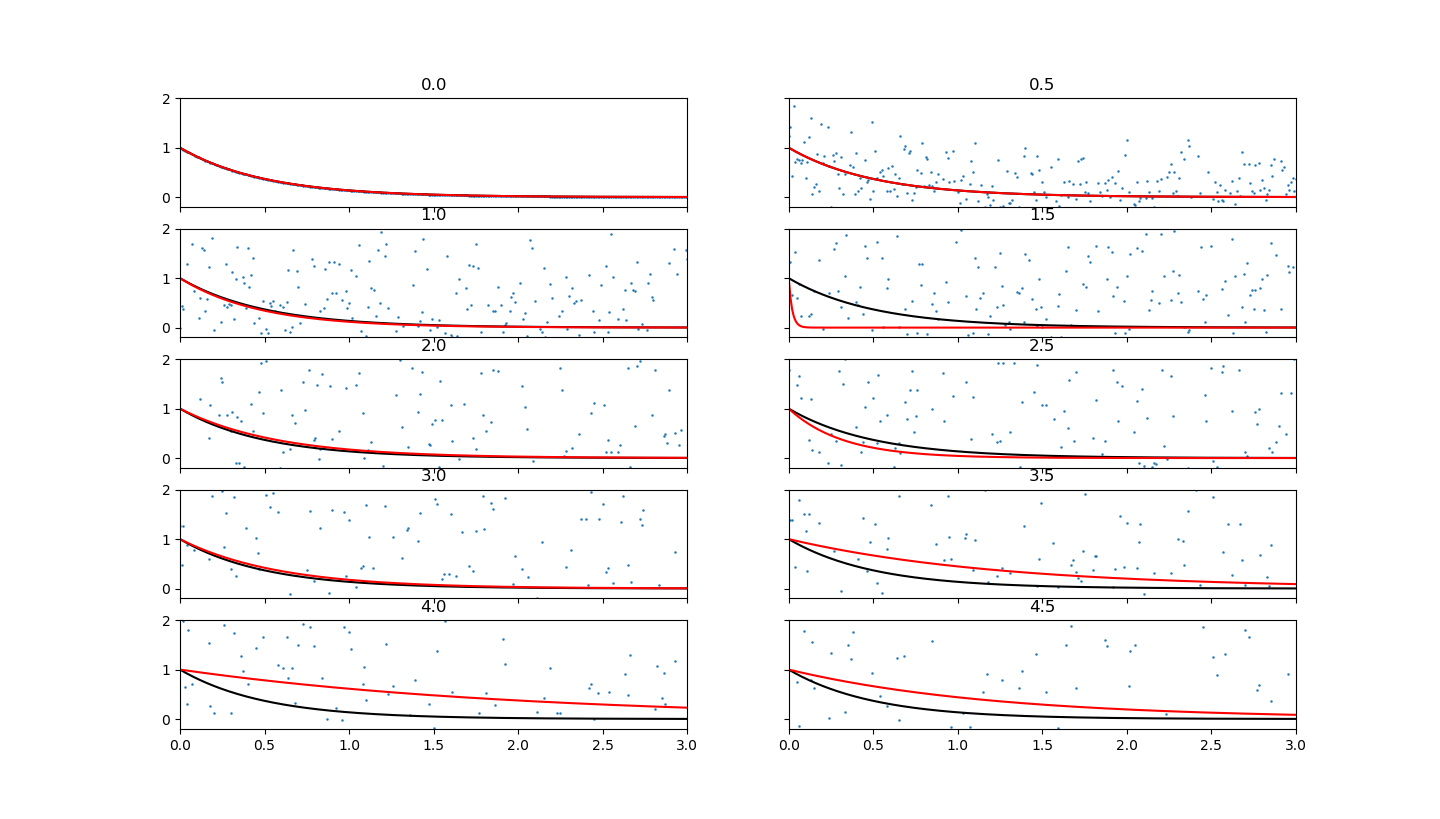
\includegraphics[width=1\textwidth]{Q1132.png}
\caption{Données, courbe théorique (noire) et simulée (rouge) pour $a=2$ et différentes valeurs de $b  \in [0,5]$ par 0.5. Avec condition d'arrêt fixée par rapport au nombre d'itérations et à la norme du gradient avec $k = 10000$ et $|g|=0.01$.}
\label{FigQ1132}


\end{figure}

On constate que pour $b$ supérieur à 1, la prédiction devient chaotique,  dans certains cas seulement. Ainsi le $a$ prédit peut être éloigné du $a$ réel et dans d'autre cas relativement proche du $a$ théorique (cas où $b = 4$). L'absence de converge vers le modèle théorique peut s'expliquer par  l'effet SCE à l'initiation et la distribution des $y_i$. En effet rappelons que $\frac{d f}{d a} = \sum_{i=1}^N (y_i - e^{-ax_i})(x e^{-ax_i})$, donc selon la distribution des $y_i$ la $dLM$ peut être fortement influencé, et l'estimation du paramètre $a$ rapidement biaisé. De plus la SCE augmente avec $b$. Toutefois cette seule explication n'est satisfaisante étant donné les résultats obtenus pour $b=1.5$ [\ref{FigQcap}]. Il pourrait s'agir d'un défaut d'implémentation de l'algorithme \vreb|LM|.


  \begin{figure}[H]
\centering
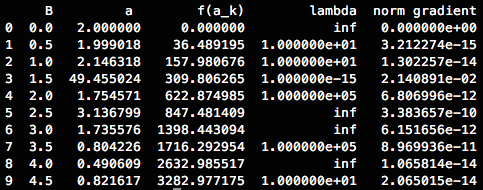
\includegraphics[width=1\textwidth]{Q113CAP.png}
\caption{Résultats numériques obtenu à la fin du processus pour les figures [\ref{FigQ1132}] .}
\label{FigQcap}
\end{figure}
 
 \section*{\color{brick} Cas 2:  Fonction bi-exponentielle}
 \textbf{\color{brick}1.} Nous travaillons sur la fonction $g(x) = x^a1 e^{-a2x}$. Comme précédemment les images $g$ renvoyé par la fonction \verb|g2(x,a1,a2)|, qui prend en entrée un vecteur \verb|x| et les valeurs des paramètres.\\
 Nous constituons un jeu de donnée à partir de cette $g(x)$ via la fonction\\
 \verb|random\_data\_set2(x,a1,a2,b)|  qui prend en entrée un vecteur x, dans l'exercice $x \in [0,5]$, les valeurs des paramètre ici $a1 = 2$ et $a2 =3$, et bruit b, on prendra pour le test $b=0.01$.
 
 
  \begin{figure}[H]
\centering
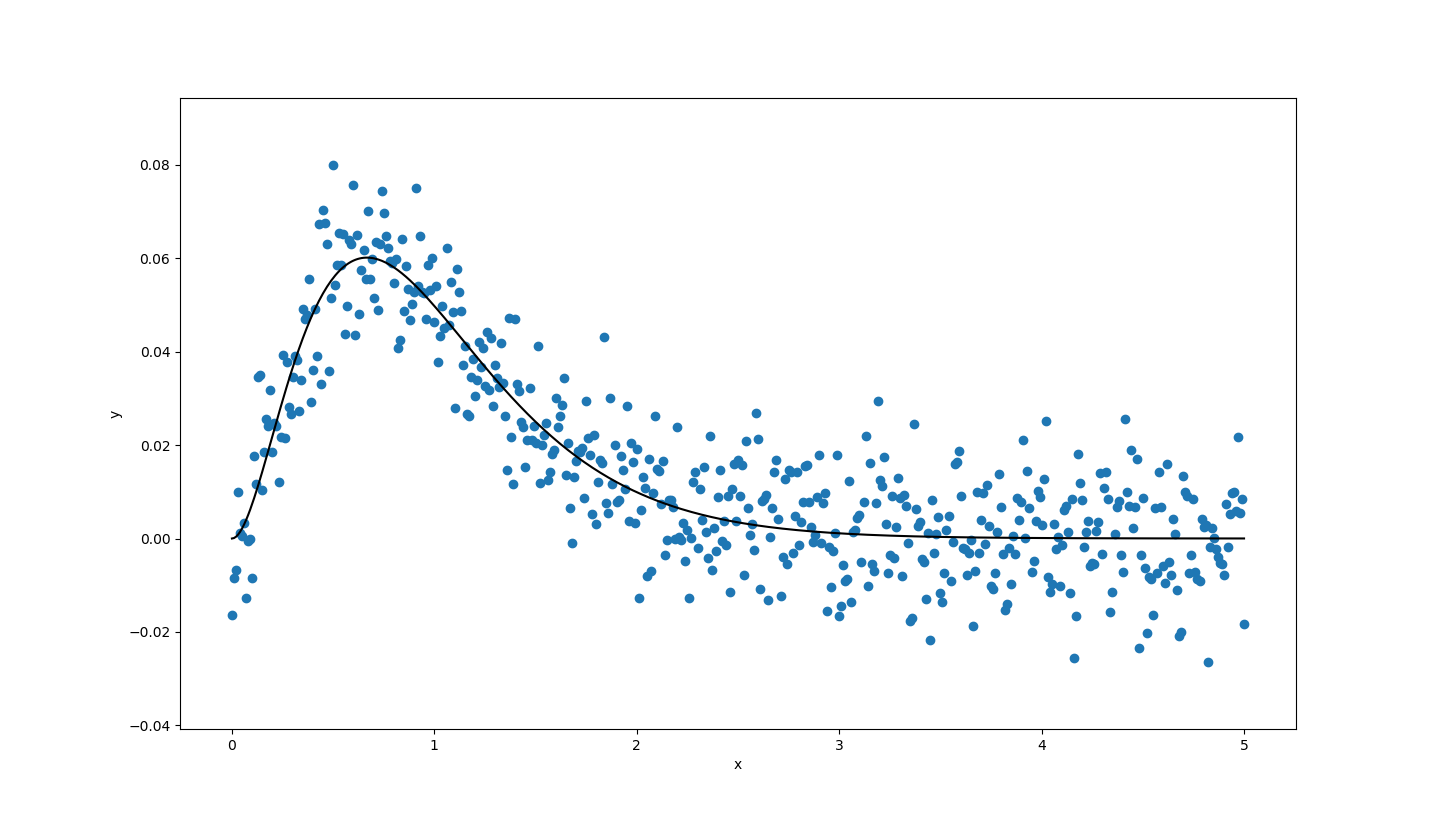
\includegraphics[width=0.7\textwidth]{Q12.png}
\caption{Représentation du jeu de données et de la courbe théorique $g(x)= x^{a1}e^{-a2x}$.}
\label{FigQ12}
\end{figure}

 \textbf{\color{brick}2 .} L'expression du gradient de $f$ par rapport à $a$ est :
 \begin{align*}
     \frac{\partial f}{\partial a1} &= -\sum_{i=1}^N (y_i - x_i^{a1}e^{-a2x})\frac{\partial g}{\partial a_1} \\
     &= -\sum_{i=1}^N (y_i - x_i^{a1}e^{-a2x})(ln(x)x^{a1}e^{-a2x})
 \end{align*}{}
  \begin{align*}
     \frac{\partial f}{\partial a2} &= -\sum_{i=1}^N (y_i - x_i^{a1}e^{-a2x})\frac{\partial g}{\partial a_2} \\
     &= -\sum_{i=1}^N (y_i - x_i^{a1}e^{-a2x})(-x^{a_1+1}e^{-a2x})
 \end{align*}{}
 
 Le gradient de la fonction f est donné par \verb|grad2 (x,y,a1,a2)| qui renvoie à partir d'un jeu de données contenues dans le vecteur \verb|y| d'un intervalle \verb|x| et de deux paramètre, $\nabla f$ un vecteur de dimension 2.
 
 
  \textbf{\color{brick}3 .} Calculons la dérivées seconde de la fonction $f$ par rapport $a_1$ et $a_2$ :
  $$H = \begin{pmatrix} 
\frac{\partial^2 f}{\partial x^2} & \frac{\partial^2 f}{\partial x\partial y} \\
\frac{\partial^2 f}{\partial x \partial y} & \frac{\partial^2 f}{\partial y^2} \\
\end{pmatrix} =
\begin{pmatrix} 
\sum_{i=1}^N (ln(x) x^{a_1} e^{-a2x})^2 & \sum_{i=1}^N (ln(x) x^{a_1} e^{-a2x})(-x^{a_1+1}e^{-a2x})  \\
 \sum_{i=1}^N (ln(x) x^{a_1} e^{-a2x})(-x^{a_1+1}e^{-a2x}) & \sum_{i=1}^N (-x^{a_1+1}e^{-a2x})^2 \\
\end{pmatrix}
$$

Nous avons ici calculé la dérivée seconde par l'approximation de Newton. De plus dans notre cas nous allons multiplier la matrice Hessienne par $(1 + \lambda)$ pour favoriser les termes diagonaux si $\lambda$ est grand et donc l'importance de la dérivée première par rapport à la dérivée seconde et réciproquement si $\lambda$ est petit. On obtient :
$$HLM = 
\begin{pmatrix} 
\sum_{i=1}^N (ln(x) x^{a_1} e^{-a2x})^2 & \sum_{i=1}^N (ln(x) x^{a_1} e^{-a2x})(-x^{a_1+1}e^{-a2x})  \\
 \sum_{i=1}^N (ln(x) x^{a_1} e^{-a2x})(-x^{a_1+1}e^{-a2x}) & \sum_{i=1}^N (-x^{a_1+1}e^{-a2x})^2 \\
\end{pmatrix} (1 +\lambda)
$$
 
 Cette matrice est calculée grâce à la fonction \verb|derivative_2_f2(x,y,a1,a2, l)|, ici l représente la valeur de $\lambda$.
 
 \textbf{\color{brick}4 .}
Dans le cas bi-exponentielle la méthode de Levenberg Marquardt est contenu dans la fonction \verb|LM2 (x,y,a1, a2,l,cond, k, g)|. Cette fonction à les mêmes étapes de calcul que celles décrites précedemment mais fait appels aux sous-fonctions :
\begin{itemize}
    \item \verb|grad2| pour le calcul du gradient 
    \item \verb|derivative_2_f2| pour le calcul du gradient pour le calcul de la Hessienne
    \item \verb|stop| pour la condtions d'arrêt
\end{itemize}
La fonction \verb|LM2| retourne 5 listes : L=> $\lambda$, G=> $|\nabla f|$ , A1 => $a1_k$ , et A2 => $a2_k$.\\
Pour un intervalle $x\in [0,5]$, des paramètres égaux à $a_1 = 2 $ et  $a_2 = 3 $,  un bruit $b =0.01$, et la double condition d'arrêt on obtient les résutats suivant:
 
  
 \begin{figure}[H]
\centering
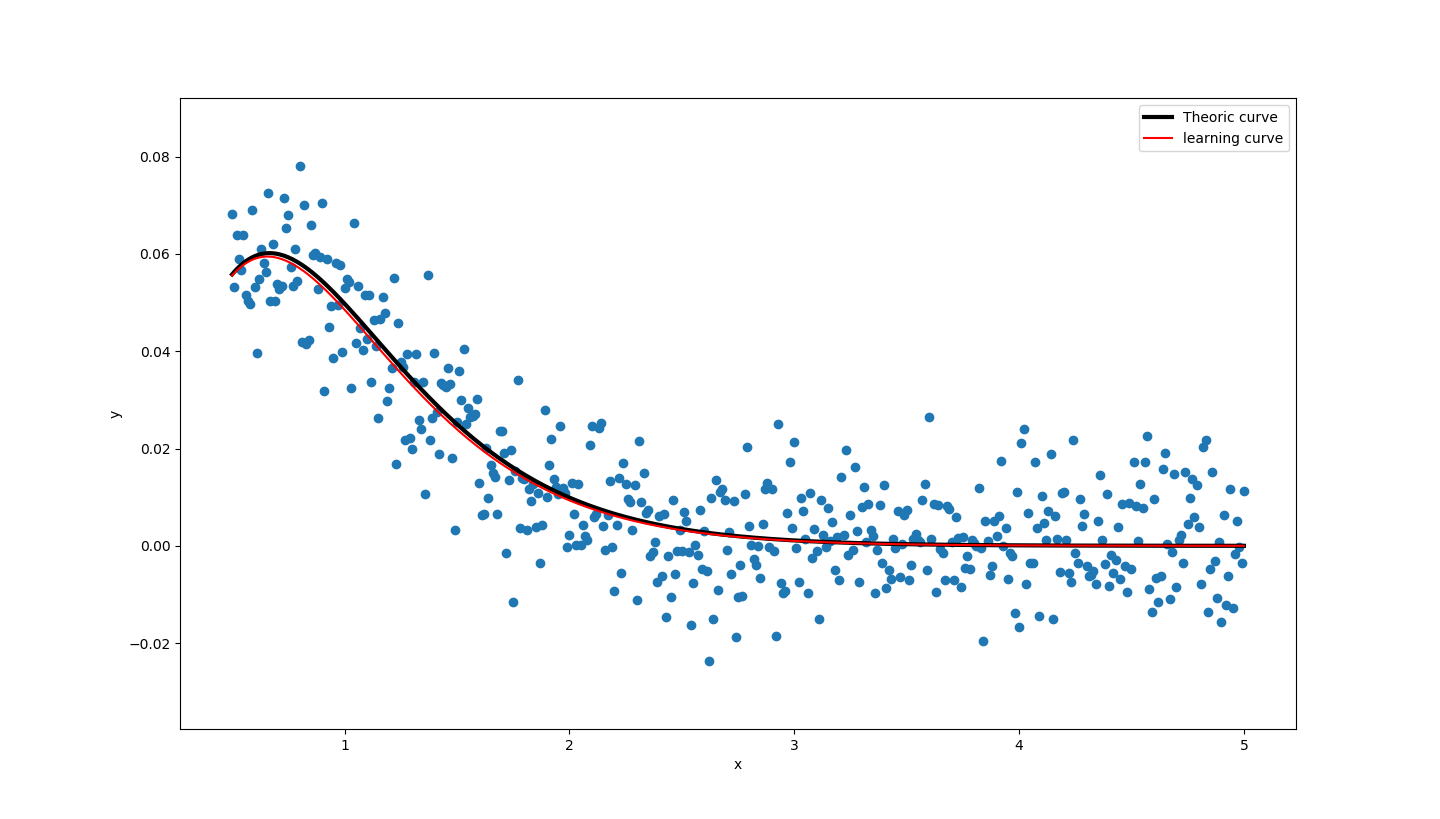
\includegraphics[width=1\textwidth]{Q15.png}
\caption{Représentation du jeu de données et de la courbe théorique $g(x)= x^{a1}e^{-a2x}$ en noire et de la courbe issue des approximation de $a_1$ et $a_2$ e rouge.}
\label{FigQ12}
\end{figure}
 
 \textbf{\color{brick}5 .} Nous allons observer l'évolution de $\lambda$, de $|\nabla f|$ et de la fonction de coût au cours des itérations, pour $g(x)=x^{a1}e^{-a2x} $, $b=0.01$ aevc un jeu de données de 100 points, et des paramètres initiaux tels que $a_{1|k=0}=1.5$ et $a_{2|k=0}=1.5$ . 
 
  \begin{figure}[H]
\centering
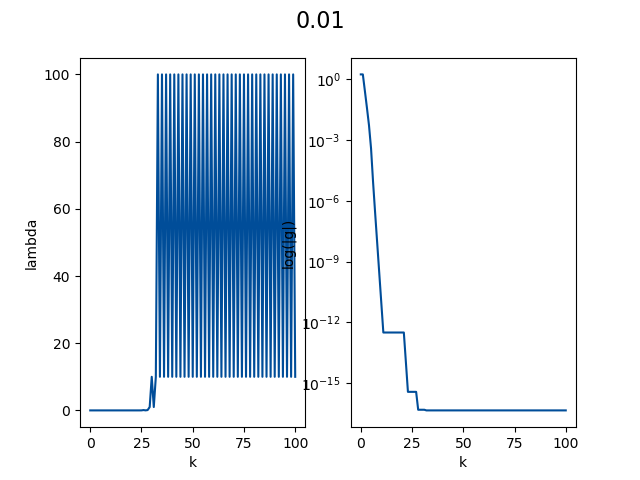
\includegraphics[width=0.8\textwidth]{Q161.png}
\caption{Variation du paramètre $\lambda$ et du logarithme de la norme euclidienne  de $\nablaf$}
\label{FigQ12}
\end{figure}
 
 Le paramètre $\lambda$ oscille entre 10 et 100, le gradient quant à lui décroît au cours des itérations et un plateau à $10^-15$
  
   \begin{figure}[H]
\centering
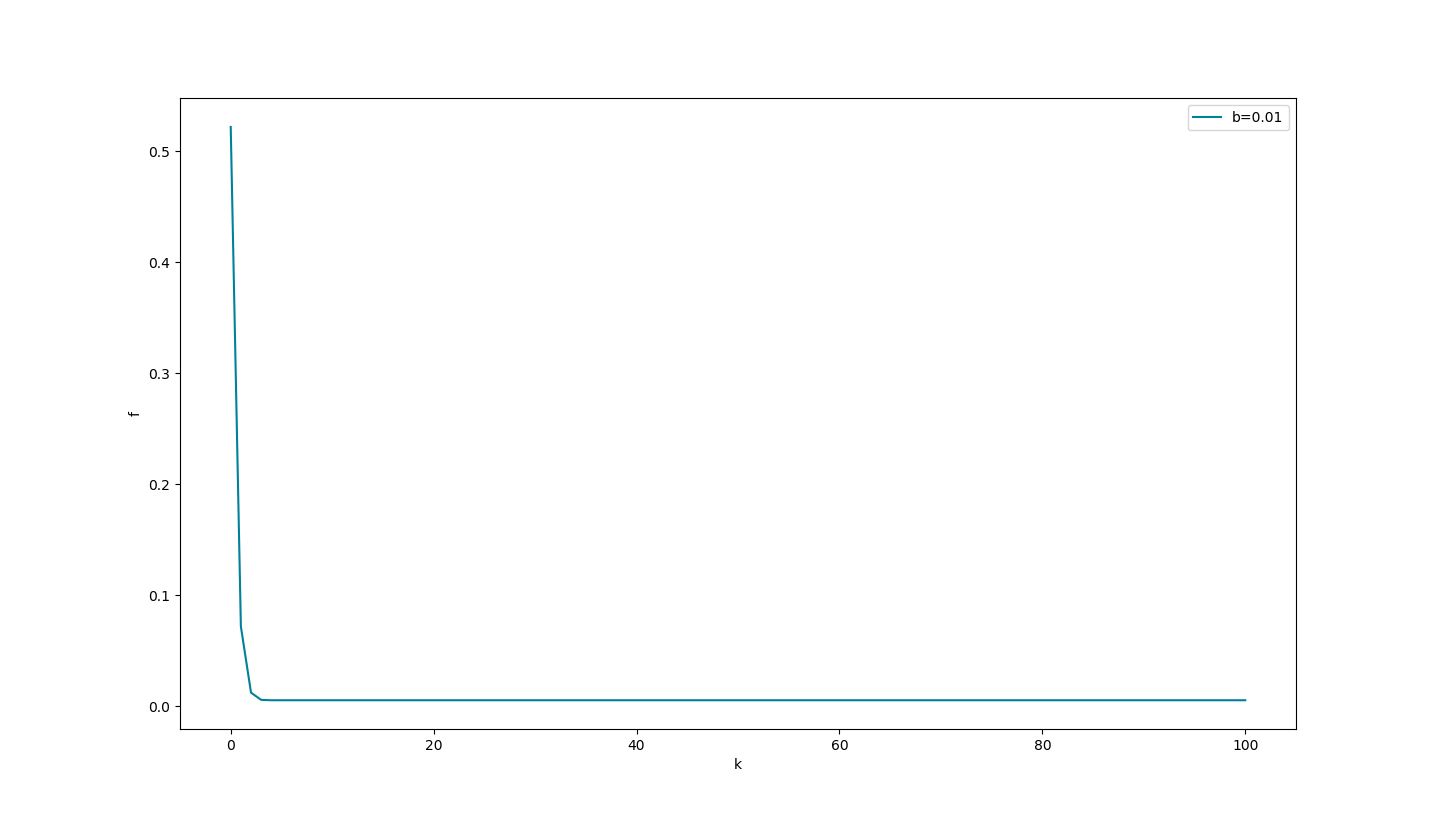
\includegraphics[width=0.8\textwidth]{Q162F.png}
\caption{Évolution de la fonction de coût $f(a_1, a_2)$.}
\label{FigQ162F}
\end{figure}

Ici comme le brui est très faible, $b=0.01$, la SCE minimale est proche de 0. D'après le graphique \ref{FigQ162F}  l'algorithme \verb|LM2| converge en 3 itérations vers ce minimum.

   \begin{figure}[H]
\centering
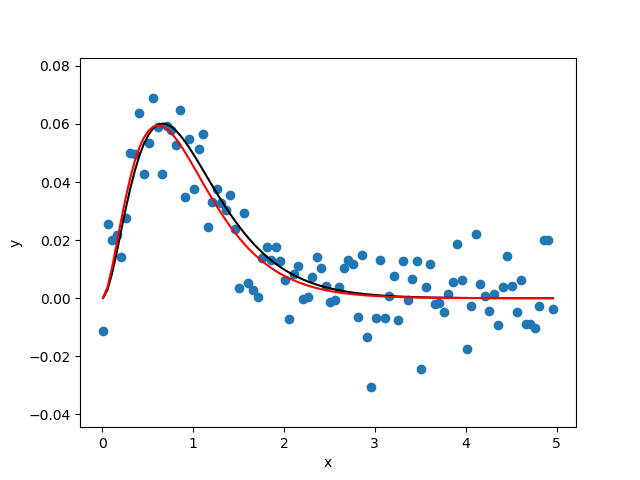
\includegraphics[width=0.7\textwidth]{Q163.png}
\caption{Résultats de l'algorithme 'LM2' pour les conditions de la questoin 11, avec les approximations : $\hat{a_1}= 1.83$ et $\hat{a_2}= 3.08$, sachant que la condition d'arrêt a été par le nombre d'itérations tel que $k=100$ .}
\label{FigQ162F}
\end{figure}

   \end{document}
  